\documentclass[12pt]{article}
% my packages
\usepackage{fullpage}
\usepackage{graphicx}
\usepackage{amsmath}
\usepackage{amsthm}
\usepackage{amssymb}
\usepackage{mathtools}
\usepackage{verbatim}
\usepackage{color}
\usepackage{boxedminipage}
\usepackage{slashbox}
\usepackage{enumitem}
\usepackage[caption=false]{subfig}
\usepackage{url}
\usepackage{listings}
\usepackage{xcolor}
\usepackage{hyperref}

\definecolor{commentcolor}{rgb}{0,0.6,0}
\definecolor{keywordcolor}{rgb}{0,0,0.8}
\definecolor{numbercolor}{rgb}{0.5,0.5,0.5}
\definecolor{stringcolor}{rgb}{0.58,0,0.82}
\lstset{%
    language=Verilog,                        % closest to BSV
    backgroundcolor=\color{white},           % choose the background color; you must add \usepackage{color} or \usepackage{xcolor}
    basicstyle=\ttfamily\bfseries,              % the size of the fonts that are used for the code
    belowskip=0.5\baselineskip,            % from: http://tex.stackexchange.com/questions/118730/avoid-empty-vert-space-after-lstlisting
    breakatwhitespace=false,                 % sets if automatic breaks should only happen at whitespace
    breaklines=true,                         % sets automatic line breaking
    captionpos=b,                            % sets the caption-position to bottom
    commentstyle=\color{commentcolor},       % comment style
    deletekeywords={...},                    % if you want to delete keywords from the given language
    escapeinside={\%*}{*)},                  % if you want to add LaTeX within your code
    extendedchars=true,                      % lets you use non-ASCII characters; for 8-bits encodings only, does not work with UTF-8
    frame=single,                            % adds a frame around the code
    %frame=none,                              % doesn't add a frame around the code
    keepspaces=true,                         % keeps spaces in text, useful for keeping indentation of code (possibly needs columns=flexible)
    %columns=fixed,                           %
    columns=flexible,                        %
    keywordstyle=\color{keywordcolor},       % keyword style
    morekeywords={%
        call,%Called method
        def,%Defined method
        inverted,%Inverted interface
        type,typedef,valueOf,                                    % Type related keywords
        method,endmethod,action,endaction,                  % Methods and actions
        Action,ActionValue,interface,endinterface,          % Interfaces
        Vector,replicate,replicateM,                        % Vector stuff
        Bit,Int,UIng,Reg,Integer,let,tagged,union,struct,   % Basic types
        TAdd,TMul,TDiv,                                     % Type operations
        rule,endrule,return,                                % Rules keywords
        pack,unpack,zeroExtend,signExtend,                  % Common bit functions
        case,matches,endcase                                % Case statements
        synthesize,True,False,Empty,*,...},                 % Etc.
    numbers=left,                            % where to put the line-numbers; possible values are (none, left, right)
    numbersep=5pt,                           % how far the line-numbers are from the code
    numberstyle=\tiny\color{numbercolor},    % the style that is used for the line-numbers
    rulecolor=\color{black},                 % if not set, the frame-color may be changed on line-breaks within not-black text (e.g. comments (green here))
    showspaces=false,                        % show spaces everywhere adding particular underscores; it overrides 'showstringspaces'
    showstringspaces=false,                  % underline spaces within strings only
    showtabs=false,                          % show tabs within strings adding particular underscores
    stepnumber=1,                            % the step between two line-numbers. If it's 1, each line will be numbered
    stringstyle=\color{stringcolor},         % string literal style
    tabsize=2,                               % sets default tabsize to 2 spaces
    title=\lstname                           % show the filename of files included with \lstinputlisting; also try caption instead of title
}

\newcommand{\mycomment}[1]{\emph{\textcolor{red}{[#1]}}}

\newcommand{\code}[1]{\texttt{#1}}
\newcommand{\inst}[1]{\textsf{#1}}

\begin{document}

\title{RiscyOO Design Document}
\author{Sizhuo Zhang \\ szzhang@csail.mit.edu \\ MIT CSAIL}
\date{}
\maketitle

\section{Overview}


\section{Processor Core}

Figure~\ref{fig:core} shows the overall structure of the processor core.
Modules are represented by boxes.
The main processor pipeline is the following:
\begin{itemize}
    \item Fetch pipeline $\rightarrow$ Rename stage $\rightarrow$ ROB and all execution pipelines (ALU/Branch, FPU/Int-Mul/Int-Div, and Mem) $\rightarrow$ Commit stage.
\end{itemize}
The rename stage divides the processor core into the front-end and the back-end.
The front-end, i.e., the fetch pipeline, is an in-order pipeline, while out-of-order execution happens all in the back-end.

An instruction is fetched and decoded in the fetch pipeline.
The rename stage performs register renaming and enters the instruction int ROB and one of the execution pipelines.
When the instruction finishes execution and leaves the execution pipeline, it notifies the ROB that it is executed.
Finally the commit stage commits instructions from ROB in order.

Below we introduce some basic information about the core, which is not tied to each specific module.

\noindent\textbf{Superscalarity:}
The processor core is also superscalar.
The fetch pipeline, rename stage and commit stage can all handle multiple instructions in one cycle.
\emph{The size of superscalarity is represented by numeric type \code{SupSize} in the source code and in the rest of this document.}
The core also has multiple execution pipelines.
The numbers of ALU/Branch (abbreviated as ALU in the following) execution pipelines and FPU/Int-Mul/Int-Div execution pipelines (abbreviated as FPU in the following) are parametrized.
However, there can only be one memory execution pipeline

\begin{figure}
    \centering
    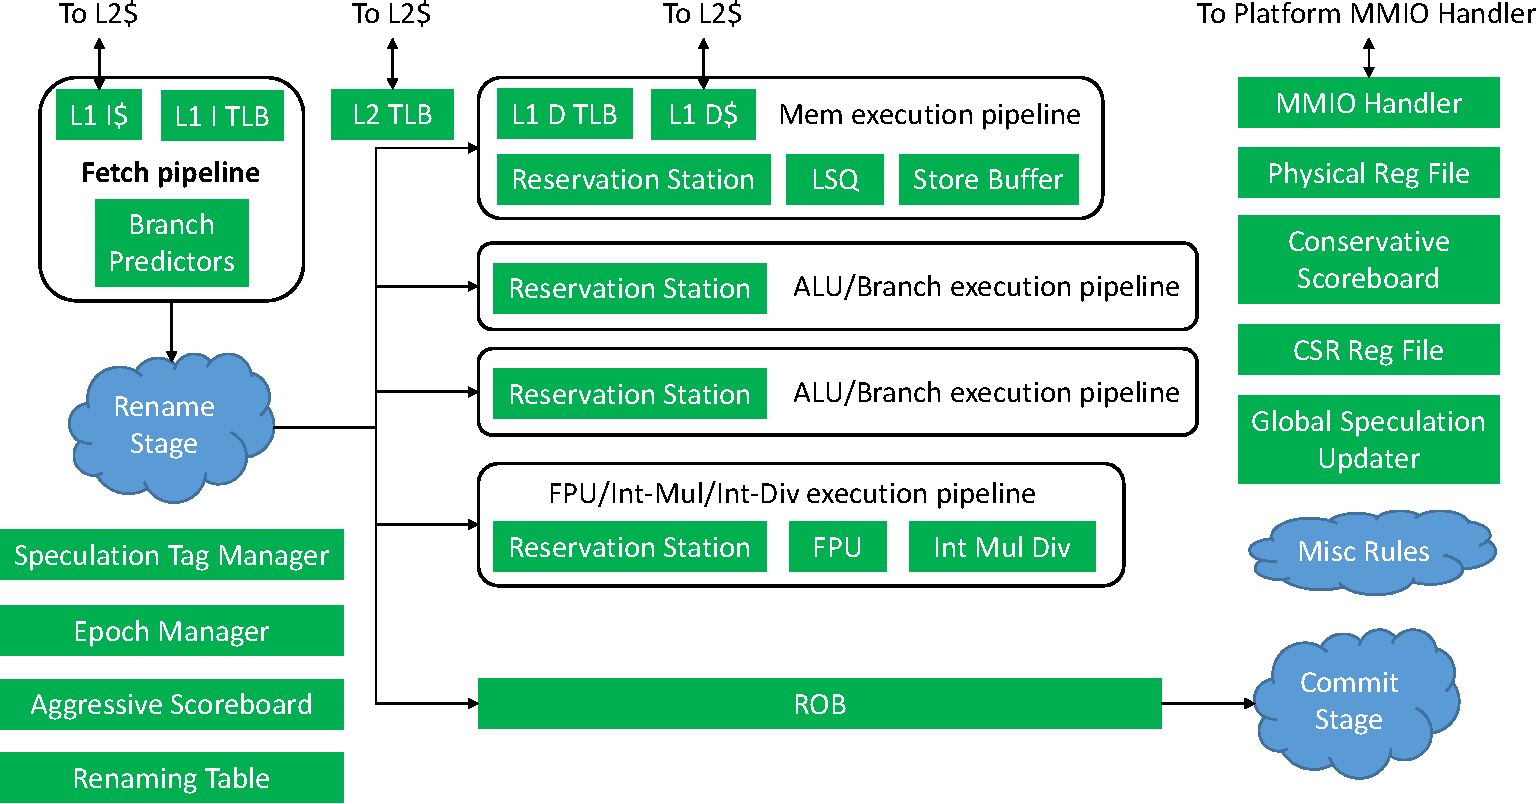
\includegraphics[width=\columnwidth]{fig/core_crop.pdf}
    \caption{Overall structure of the processor core}\label{fig:core}
\end{figure}

\noindent\textbf{Scheduling Convention:}
Since there are many modules in the core, assigning conflict matrices to different module interfaces to maximize the concurrency of rules can be difficult.
To simplify the problem, we following the convention of \emph{reverse pipeline ordering} in assigning conflict matrices.
\emph{That is, rules representing later stages in the processor pipeline (e.g., commit) are ordered before rules representing earlier stages (e.g., rename), and thus, interface methods called in later stages are ordered before methods called in earlier stages.}

\noindent\textbf{System Instructions:}
Some instructions can change the context of the processor and are difficult to be executed out of order or concurrently with other instructions.
These instructions are called \emph{system instructions}, and include the following instructions:
\begin{itemize}
    \item \inst{ECALL} which makes a system call,
    \item \inst{EBREAK} which traps for debugger,
    \item \inst{SRET} and \inst{MRET} which return from trap handling,
    \item \inst{SFENCE.VMA} which flushes the TLBs, and
    \item \inst{FENCE.I} which is used for self-modifying code.
\end{itemize}
System instructions are executed in a blocking way, i.e., the instruction will be the only instruction in the ROB.


\noindent\textbf{Detecting Interrupt:}

\noindent\textbf{Read-After-Write Hazards for CSRs:}

\noindent\textbf{Organization:}
In the rest of this section, we first introduce the general mechanism to control speculation in the back-end (Section~\ref{sec:specupdate}), and then describe each modules and top-level rules.

\subsection{Managing Speculative and Wrong-Path Instructions}\label{sec:specupdate}

Almost all instructions in the processor are speculative and may be at the wrong path, so we need to have some way to manage speculation and squash wrong-path instructions.
Since the front-end is in-order while the back-end is out-of-order, we use different schemes in the front-end and the back-end, and we explain each of the schemes next.

\subsubsection{Front-End}
The rename stage kills wrong-path instructions from the front-end (i.e., the fetch pipeline) based on the epoch in the \emph{epoch manager} (Section \mycomment{XXX}).
The fetch pipeline contains a copy of the epoch, and every fetched instruction will carry the epoch value.
At the rename stage, instructions with epochs not equal to the epoch value in the epoch manager are killed.
Whenever the PC register in the fetch pipeline needs to be redirected (because of branch mispredictions, exceptions, interrupts, or mis-speculative loads), the epoch in the epoch manager will be incremented either at the redirect time or slightly earlier.
When the PC in the fetch pipeline is truly redirected, the epoch copy in the fetch pipeline is also incremented.

Since there can be multiple consecutive redirections in the back-end, the epoch in the epoch manager should have multiple bits.
The epoch manager will recycle unused epoch values based on the epoch values of instructions seen at the rename stage.

\subsubsection{Back-End}
We use two approaches to perform squashes in the back-end:
\begin{enumerate}
    \item We delay the squash and redirection until the commit stage.
    At that time, we can simply kill every instruction in the back-end.
    \item We squash wrong-path instruction and redirect PC immediately when we find a redirection is needed (e.g., when a branch turns out to be mispredicted).
    The challenge is that we should squash only instruction younger than the instruction that triggers the redirection.
\end{enumerate}
We use the first approach for uncommon redirections, i.e., exceptions, interrupts, and the replay of mis-speculative loads that violate memory ordering.
We use the second approach for branch mispredictions only.
The implementation of these two approaches consists of the following three parts.

\noindent\textbf{Speculation tags and bit masks to track dependency on branches:}
To correctly kill wrong-path instructions in case of branch mispredictions, we assign a unique \emph{speculation tag} (type \code{SpecTag} in the source code) to each branch at the rename stage.
Every instruction will also be assigned with a speculation bit mask (type \code{SpecBits} in the source code) at the rename stage.
Each bit in the bit mask corresponds to a speculation tag.
If the bit is set, then the instruction should be killed in case the branch holding the speculation tag is mispredicted.
If a branch turns out to be predicted correctly, then the corresponding bit should be cleared from all instructions in the back-end. 
The \emph{speculation tag manager} (Section \mycomment{XXX}) assigns and recycles speculation tags, and also assigns speculation bit masks.

\noindent\textbf{Module interface to manipulate speculative instructions:}
Every module in the back-end that keeps speculative instructions should also keep the speculation bit mask for each instruction.
The module also needs to provide interface methods to allow top-level rules to squash speculative instructions or clear speculation bit masks.
All modules that keep speculative instructions except ROB provides the \code{SpeculationUpdate} interface in Figure~\ref{fig:specupdate-ifc}.
ROB provides the \code{ROB\_SpeculationUpdate} interface in Figure~\ref{fig:specupdate-ifc}.

In both interfaces, method \code{correctSpeculation} clears the speculation bit mask of each instruction in the module saccording to argument \code{mask}.
This method is called when a branch resolves to be predicted correctly.
Since multiple branches can be resolved (to be predicted correctly) in the same cycle, we use argument \code{mask} to encode the speculation tags of all these branches.

In both interfaces, method \code{incorrectSpeculation} squashes wrong-path instructions.
If argument \code{kill\_all} is true, then all instructions in the module are squashed.
This happens when commit stage commits an exception, or an interrupt, or a load that violates memory ordering.
Otherwise, only instructions whose speculation bit mask contains the speculation tag in argument \code{spec\_tag} will be squashed.
This happens when a branch is resolved and turns out to be mispredicted.
It should be noted that there can only be one source of squashing in each cycle.
In case of the ROB module, the third argument \code{inst\_tag} is the ROB index of the mispredicted branch.
It is used to simplify the squashing logic in ROB.

\begin{figure}
\begin{lstlisting}[caption={}]
interface SpeculationUpdate;
  method Action incorrectSpeculation(Bool kill_all, SpecTag kill_tag);
  method Action correctSpeculation(SpecBits mask);
endinterface
interface ROB_SpeculationUpdate;
  method Action incorrectSpeculation(Bool kill_all, SpecTag spec_tag, InstTag inst_tag);
  method Action correctSpeculation(SpecBits mask);
endinterface
\end{lstlisting}
\caption{Interface methods to manipulate speculation bit masks of modules that keep speculative instructions}\label{fig:specupdate-ifc}
\end{figure}

\noindent\textbf{Centralized entry point for manipulating speculative instructions:}
The commit stage or the branch-resolve rule does not call directly the \code{SpeculationUpdate} interface of every module to clear speculation bit masks or squashing instructions.
Instead, they both call the interface of the \emph{global speculation updater} (Section \mycomment{XXX}), which is the centralized entry point for manipulating speculative instructions.
The global speculation updater merges requests to clear speculation bit masks and then call the \code{correctSpeculation} method of every module.
It also arbitrate between requests to squash instructions and then call the \code{incorrectSpeculation} method of every module.
To some degree, having a centralized the entry point simplifies the broadcast logic for manipulating speculative instructions.



\subsection{Epoch Manager}

The epoch manager manages the epoch that is used to kill wrong-path instructions at the rename stage.
Each time a redirection happens, the epoch is incremented by one, so the epoch value will change as follows (\code{NumEpochs} is the number of unique epoch values):
\begin{center}
    0 $\rightarrow$ 1 $\rightarrow$ $\cdots$ $\rightarrow$ \code{NumEpochs}$-1$ $\rightarrow$ 0 $\rightarrow$ $\cdots$
\end{center}
The module also tracks the range of epoch values being used by instructions in the fetch pipeline.
The epoch cannot be incremented if the next epoch value falls within the range.
The range is updated by looking at the epochs of instructions coming out of the fetch pipeline.

\subsubsection{Interface}
Figure~\ref{fig:epoch-ifc} shows the interface of the epoch manager.
Now we explain each interface method:
\begin{itemize}
    \item Subinterface \code{checkEpoch}: provides a vector of methods for the rename stage to check if an instruction is at the wrong path.
    The input argument \code{e} is the epoch carried by the instruction.
    The method compares \code{e} with the internal epoch of the module, and returns false if the instruction is at the wrong path and should be killed.
    
    \item Subinterface \code{updatePrevEpoch}: provides a vector of methods to update the latest epoch values seen from the fetch pipeline.
    Every instruction that arrives at the rename stage (including wrong-path instructions) will call this method to help the module recycle unused epoch values.
    
    \item Method \code{incrementEpoch}: is called when PC needs to be redirect.
    This method increased the internal epoch of the module.
    The guard will be false if the next value of the epoch is not yet recycled (i.e., still being used by instructions in the fetch pipeline).
\end{itemize}

\begin{figure}
\begin{lstlisting}[caption={}]
interface EM_checkEpoch;
  method Bool check(Epoch e);
endinterface
interface EM_updatePrevEpoch;
  method Action update(Epoch e);
endinterface
interface EpochManager;
  interface Vector#(SupSize, EM_checkEpoch) checkEpoch;
  interface Vector#(SupSize, EM_updatePrevEpoch) updatePrevEpoch;
  method Epoch getEpoch;
  method Action incrementEpoch;
endinterface
\end{lstlisting}
\caption{Interface of epoch manager}\label{fig:epoch-ifc}
\end{figure}

\noindent\textbf{Conflict Matrix:}
The conflict matrix of the interface methods is:
\begin{enumerate}
    \item \code{checkEpoch} $<$ \code{incrementEpoch}
    \item \code{updatePrevEpoch} CF \{\code{checkEpoch}, \code{incrementEpoch}\}
\end{enumerate}
We make method \code{updatePrevEpoch} conflict free with other methods, because the recycle of unused epoch values does not need to happen immediately.

\subsubsection{Implementation}
The module has two internal registers \code{curr\_epoch} and \code{prev\_checked\_epoch}.
\code{curr\_epoch} is the current epoch value which is used to kill wrong-path instructions at the rename stage.
\code{prev\_checked\_epoch} is the last seen epoch value from the fetch pipeline.
Thus, the range of epoch values being used is: \code{prev\_checked\_epoch}, \code{prev\_checked\_epoch}$+1$, $\ldots$, \code{curr\_epoch}.

Methods \code{checkEpoch} and \code{incrementEpoch} access directly the registers.
For subinterface \code{updatePrevEpoch}, we first capture its arguments in wires, and then update the \code{prev\_checked\_epoch} register.
Wires are ok because \code{updatePrevEpoch} is conflict free with other methods.

\subsubsection{Source Code}
See module \code{mkEpochManager} in \code{//procs/lib/EpochManager.bsv}.        


\subsection{Speculation Tag Manager}\label{sec:spectag}

The speculation tag manager manages all the speculation tags (including both assigned tags and free tags).
Speculation tags are checked out or assigned at rename stage, and freed when the branch resolves in the ALU execution pipeline.
It should be noted that if a branch is mispredicted, then the speculation tags of itself and younger branches are all freed.
Since the module tracks all the in-flight speculation tags, it also assigns speculation bit mask to each instruction at the rename stage.

\subsubsection{Interface}

Figure~\ref{fig:spectag-ifc} shows the interface of the speculation tag manager.
Now we explain each interface method:
\begin{itemize}
    \item Method \code{currentSpecBits}: returns the speculation bit mask that should be assigned to the instruction at the rename stage.
    
    \item Method \code{nextSpecTag}: returns the speculation tag to be checked out for a new branch instruction at the rename stage.
    The guard is false if all tags have been checked out.
    
    \item Method \code{claimSpecTag}: checks out a new speculation tag for a new branch instruction at the rename stage.
    The guard is false if all tags have been checked out.
    
    \item Method \code{canClaim}: returns the guard of methods \code{nextSpecTag} and \code{claimSpecTag}.
    
    \item Subinterface \code{specUpdate}: See Section~\ref{sec:specupdate}.
\end{itemize}

\begin{figure}
\begin{lstlisting}[caption={}]
interface SpecTagManager;
  method SpecBits currentSpecBits;
  method SpecTag  nextSpecTag;
  method Action   claimSpecTag;
  method Bool     canClaim;
  interface SpeculationUpdate specUpdate;
endinterface
module mkSpecTagManager(SpecTagManager);
  // module implementation
endmodule
\end{lstlisting}
\caption{Interface of speculation tag manager}\label{fig:spectag-ifc}
\end{figure}

\noindent\textbf{Conflict Matrix:}
The conflict matrix of the interface methods is:
\begin{itemize}
    \item \{\code{currentSpecBits}, \code{nextSpecTag}, \code{canClaim}\} $<$ \code{claimSpecTag} $<$ \code{correctSpeculation}
    \item \{\code{currentSpecBits}, \code{nextSpecTag}, \code{canClaim}\} $<$ \code{incorrectSpeculation}
    \item \code{claimSpecTag} C \code{incorrectSpeculation}
\end{itemize}
We make \code{claimSpecTag} conflict with \code{incorrectSpeculation}, because the \code{claimSpecTag} must be called by a wrong-path instruction if \code{incorrectSpeculation} is called in the same cycle.

\subsubsection{Implementation}
The module uses EHR \code{current\_spec\_bits\_ehr} to keep the current speculation bit mask.
Each bit in the mask represents if the corresponding speculation tag is held of an in-flight branch in the ROB.
The module uses a vector of registers \code{dependent\_checkpoints} to track the dependencies between speculation tags.
\code{dependent\_checkpoints[t]} is the speculation bit mask that encodes all the speculation tags that is checked out after speculation tag \code{t} (including \code{t} also).
That is, if the branch with speculation tag \code{t} is mispredicted, then all speculation tags encoded in \code{dependent\_checkpoints[t]} should be freed.

All methods access the EHR or registers directly according to the conflict matrix.
We manually create a conflict between \code{claimSpecTag} and \code{incorrectSpeculation}.

\subsubsection{Source Code}
See module \code{mkSpecTagManager} in \code{//procs/lib/SpecTagManager.bsv}.


\subsection{Global Speculation Updater}\label{sec:globalspec}

The global speculation updater is the centralized point for calling the \code{SpeculationUpdate} interface of every module.

\subsubsection{Interface}
Figure~\ref{fig:globalspec-ifc} shows the interface of the module.
The module takes in two interface arguments.
Argument \code{ifc} is the aggregated interface of the \code{SpeculationUpdate} interface of every module.
That is, calling any method in \code{ifc} is effectively calls the corresponding method in the \code{SpeculationUpdate} interface of every module.
Argument \code{rob} is the \code{ROB\_SpeculationUpdate} method of ROB (Sections~\ref{sec:specupdate}).
The two arguments together contain all the interface methods to squash all the speculative instructions and clear all the speculation bit masks.
Now we explain each interface method returned by the module:
\begin{itemize}
    \item Subinterface \code{correctSpec}: provides a vector of methods to clear bits in every speculation bit mask in the back-end.
    This method is called when branch resolves to be predicted correctly.
    Having a vector of methods allows multiple branches to be resolved in one cycle.
    \item Method \code{incorrectSpec}: squashes speculative instructions by calling the\\ \code{incorrectSpeculation} method of every module in the back-end.
\end{itemize}

\begin{figure}
\begin{lstlisting}[caption={}]
interface GlobalSpecUpdate#(numeric type correctSpecPortNum, numeric type conflictWrongSpecPortNum);
  interface Vector#(correctSpecPortNum, Put#(SpecTag)) correctSpec;
  method Action incorrectSpec(Bool kill_all, SpecTag spec_tag, InstTag inst_tag);
endinterface
module mkGlobalSpecUpdate#(
  SpeculationUpdate ifc, ROB_SpeculationUpdate rob
)(GlobalSpecUpdate#(correctSpecPortNum, conflictWrongSpecPortNum));
  // module implementation
endmodule
\end{lstlisting}
\caption{Interface of global speculation updater}\label{fig:globalspec-ifc}
\end{figure}

\noindent\textbf{Conflict Matrix:}
The conflict matrix of the interface methods is:
\begin{itemize}
    \item \code{correcSpec[i]} CF \code{correctSpec[j]}
    \item \code{correctSpec} C \code{incorrectSpec}
    \item \code{incorrectSpec} C \code{incorrectSpec}
\end{itemize}
Note that method \code{incorrectSpec} is conflict with itself, so there can only be one rule calling it to squash instructions in each cycle.

There is no very specific reason for making \code{correctSpec} conflict with \code{incorrectSpec}.
Making conflicting may reduce the amount of data being broadcast, otherwise we need to broadcast \code{SpecBits} for both \code{correctSpec} and \code{incorrectSpec}.
Making them conflict might also simplify overall scheduling.

\subsubsection{Implementation}\label{sec:globalspec:impl}
The \code{incorrectSpec} method simply calls the \code{incorrectSpeculation} method in module argument \code{ifc} and \code{rob} (in Figure~\ref{fig:globalspec-ifc}).
The \code{correctSpec} methods use wires to record their input arguments, i.e., the speculation tag to be freed.
Then, a canonicalize rule  merges all the speculation tags that are freed into a speculation bit mask and calls the \code{correctSpeculation} method in module argument \code{ifc} and \code{rob}.
We manually create conflict between \code{correctSpec} and \code{incorrectSpec}.

Currently, the \code{incorrectSpec} and \code{correctSpec} methods will broadcast to all modules in a single cycle.
This may complicate routing.
To reduce the pressure on routing, we can broadcast these methods to modules in multiple cycles (e.g., via a register pipeline).
However, we still need to make sure that the \code{correctSpeculation} or \code{incorrectSpeculation} method of all modules are called atomically in one rule.
Futhermore, when a \code{incorrectSpec} method call is being broadcast to all the modules, we should block any future calls to this module until the broadcast is done.
This is because the instruction that initiate the future call may be killed by the broadcast.

\subsubsection{Source Code}
See module \code{mkGlobalSpecUpdate} in \code{//procs/lib/GlobalSpecUpdate.bsv}.

\subsubsection{Future Improvement}
We should pipeline the broadcast as described in Section~\ref{sec:globalspec:impl}.


\subsection{Aggressive (Optimistic) Scoreboard}\label{sec:sbaggr}

The aggressive scoreboard holds an optimistic version of the presence bits of all the physical registers.
Instructions in the execution pipeline can optimistically set the presence bits in this scoreboard even when the instruction has not yet finished execution (but it may be close to finish).
The renaming stage will check the presence bits from this scoreboard for the source registers of the renaming instruction, and unset the present bit in this scoreboard for the destination register of the renaming instruction.

The interface and module presented here are slightly different from what is the source code, because the module in the source code is used for not only this aggressive scoreboard but also another conservative scoreboard (Section~\ref{sec:prf+sbcons}).

\subsubsection{Interface}
Figure~\ref{fig:aggr-sb-ifc} shows the interface of this module.
Now we explain each interface method: 
\begin{itemize}
    \item Subinterface \emph{setReady}: provides a vector of methods for instructions in execution pipelines to set the presence bits of their physical destination registers optimistically.
    \item Subinterface \emph{eagerLookup}: provides a vector of methods for instructions at the renaming stage to check the presence bits of their physical source registers.
    \item Subinterface \emph{setBusy}: provides a vector of methods for instructions at the renaming stage to unset the presence bits of their physical destination registers.
\end{itemize}

\begin{figure}
\begin{lstlisting}[caption={}]
// PhyRegs is a struct containing all the physical regs of an instruction
// RegsReady is a struct containing the presence bits for all the physical regs of an instruction
// PhyRIndex is the index of a physical reg
// SupSize is the superscalar size
interface SbLookup;
  method RegsReady get(PhyRegs r);
endinterface
interface SbSetBusy;
  method Action set(Maybe#(PhyRIndx) dst);
endinterface
interface ScoreboardAggr#(numeric type setReadyNum);
  interface Vector#(setReadyNum, Put#(PhyRIndx)) setReady;
  interface Vector#(SupSize, SbLookup) eagerLookup;
  interface Vector#(SupSize, SbSetBusy) setBusy;
endinterface
module mkScoreboardAggr(ScoreboardAggr#(setReadyNum));
  // module implementation
endmodule
\end{lstlisting}
\caption{Interface of the aggressive scoreboard}\label{fig:aggr-sb-ifc}
\end{figure}

\noindent\textbf{Conflict Matrix:}
The conflict matrix of the interface methods is:
\begin{center}
    setReady[0] $<$ $\cdots$ $<$ setReady[setReadyNum-1] $<$ eagerLookup[0] $<$ setBusy[0] $<$ eagerLookup[1] $<$ setBusy[1] $<$ $\cdots$ $<$ eagerLookup[SupSize-1] $<$ setBusy[SupSize-1].
\end{center}
We put all methods in a total order, though the conflict matrix does not need to transitive.
We order setReady $<$ eagerLookup to match the rule ordering between instruction-execution rules (which call setReady) and the renaming rule (which calls eagerLookup).
The rule ordering is because the execution rules are in later stages of the pipeline than renaming.
Thus, eagerLookup will observe the effects of all the calls to setReady in the same cycle, and this is why we call it ``eager''.
Methods eagerLookup[$i$] and setBusy[$i$] are used by the $i^{th}$ renamed instruction at the renaming stage in each cycle.
Since the $i^{th}$ instruction should see the renaming effects of all previous instructions, we order setBusy[$0\ldots i-1$] $<$ eagerLookup[$i$].

\subsubsection{Implementation}
The implementation of the module does not contain any internal rules.
It just uses a vector of EHRs to hold the presence bits, one EHR for each bit.
The interface methods access the EHRs using the appropriate port according to the conflict matrix.

\subsubsection{Source Code}
See the followings:
\begin{itemize}
    \item module \texttt{mkScoreboardAggr} in \texttt{//procs/RV64G\_OOO/ScoreboardSynth.bsv}, and
    \item module \texttt{mkRenamingScoreboard} in file \texttt{//procs/lib/Scoreboard.bsv}.
\end{itemize}
  

\subsection{Physical Register File and Conservative Scoreboard}\label{sec:prf+sbcons}

The physical register file contains the value for each physical register, and the conservative scoreboard contains the presence bit for each physical-register value.
Instructions at the renaming stage will unset the presence bits of the destination physical registers.
Instructions that just finish execution write data into the physical register file and set the presence bits simultaneously.
Instructions in the execution pipeline read both the physical register file and the scoreboard to get the source operand and whether the operand data is present or not.
The scoreboard is called conservative because each presence bit is set only when the data is written to the corresponding physical register.

Although the physical register file and the conservative scoreboard are currently implemented as two separate modules, we describe them as one module here because they should be accessed together.

\subsubsection{Interface}
Figure~\ref{fig:prf-sb-ifc} shows the interface of the fused module of the physical register file and the conservative scoreboard.
It should be noted that the interface shown here is different from what is in the source code, which splits this module as two separate modules.

\begin{figure}[!htb]
\begin{lstlisting}[caption={}]
// PhyRIndex is the index of a physical reg
// SupSize is the superscalar size
interface RFileWr;
  method Action wr(PhyRIndx rindx, Data data);
endinterface
interface RFileRd;
  method Maybe#(Data) rd1(PhyRIndx rindx);
  method Maybe#(Data) rd2(PhyRIndx rindx);
  method Maybe#(Data) rd3(PhyRIndx rindx);
endinterface
interface SbSetBusy;
  method Action set(Maybe#(PhyRIndx) dst);
endinterface
interface RFileSbCons#(numeric type wrNum, numeric type rdNum);
  interface Vector#(wrNum, RFileWr) write;
  interface Vector#(rdNum, RFileRd) read;
  interface Vector#(SupSize, SbSetBusy) setBusy;
endinterface
module mkRFileSbCons(RFileSbCons#(wrNum, rdNum));
  // module implementation
endmodule
\end{lstlisting}
\caption{Interface of physical register file and conservative scoreboard}\label{fig:prf-sb-ifc}
\end{figure}

Now we explain each interface method:
\begin{itemize}
    \item Subinterface \emph{write}: provides a vector of methods for instructions that just finish execution to write the data into the physcial register file and set the presence bit.
    \item Subinterface \emph{read}: provides a vector of methods for instructions at register-read stage to read both the data and presence bit of the source register.
    In case the presence bit is unset, the method returns \texttt{Invalid}.
    \item Subinterface \emph{setBusy}: provides a vector of methods for instructions at the renaming stage to unset the presence bits of their physical destination registers.
    this method will be called together with the one in the aggressive scoreboard.
\end{itemize}

The conflict matrix of the interface methods is:
\begin{itemize}
    \item read CF \{write, setBusy\}
    \item write[0] $<$ write[1] $<$ $\cdots$ $<$ write[wrNum-1] $<$ setBusy[0] $<$ setBusy[1] $<$ $\cdots$ $<$ setBusy[wrNum-1]
\end{itemize}
We set all the read methods conflict free with all the write methods, because reads do not need to reflect the effects of writes immediately.
In case an old instruction is writing a register which is being read by a younger instruction as a source operand, it is ok for the read method to return \texttt{Invalid} even if the write method has been called.
This simply delays the execution of the younger instruction.
In our implementation, the read method will return \texttt{Invalid} if a write for the same physical register is being performed in the same cycle.
This can cut off the combinational path.

Forcing read methods to be ordered before write methods can cause rule-scheduling problems, because rules that read the register file are in earlier pipeline stages than rules that write register file.
That is, the method ordering will not agree with the (desired) top-level rule ordering.

We also set all the read methods conflict free with all the setBusy methods.
This is because the renaming algorithm guarantees that a physical register that is being used as a source operand of a (currently correct-path) instruction cannot be a free register for renaming destination architectural registers.
However, \emph{it is still desirable in the furture implementation to set all the read methods $<$ all the setBusy methods}, because reads happen in later pipeline stages than setBusy does.

We order all the write methods before all the setBusy methods, because write methods are called in later stages in the pipeline than setBusy methods.

\subsubsection{Implementation}
The implementation uses a vector of EHRs to store the register data, and another vector of EHRs to store the presence bits.
The write methods and set busy methods directly access the EHRs using appropriate ports according to the conflict matrix of the interface.

The read methods do not directly access the EHRs.
We use a vector of wires to retrieve value of port 0 of each EHR, and the read methods read from these wires.
This prevents any combinational path from write to read.
This is a valid implementation because the read methods are conflict free with the write and setBusy methods, and the read methods can safely ignore the effects caused by the write or setBusy methods.

\subsubsection{Source Code}
See the followings:
\begin{itemize}
    \item module \texttt{mkRFileSynth} in file \texttt{//procs/RV64G\_OOO/RFileSynth.bsv},
    \item module \texttt{mkRFile} in file \texttt{//procs/lib/PhysRFile.bsv},
    \item module \texttt{mkScoreboardCons} in file \texttt{//procs/RV64G\_OOO/ScoreboardSynth.bsv}, and
    \item module \texttt{mkRenamingScoreboard} in file \texttt{//procs/lib/Scoreboard.bsv}.
\end{itemize}

\subsubsection{Future Improvement}
There are two improvements to make in a future implementation:
\begin{enumerate}
    \item Merge the physical register file and the conservative scoreboard into one module to ensure that their methods are called together.
    \item Order the read methods before the setBusy methods, so we don't need to rely on the high-level invariant of the renaming algorithm to ensure correctness.
\end{enumerate}

\subsection{ROB}\label{sec:rob}

The ROB keeps all the in-flight instructions that have been renamed but not committed.
Instructions are enqueued into ROB in order at the renaming stage, and are dequeued from the ROB in order at the commit stage.
Instructions in the execution pipeline will also access the corresponding ROB entry.

\subsection{Interface}
Before introducing the interface of the module, we first explain the fields in an ROB entry.
Figure~\ref{fig:rob-entry} shows the definition of type ToReorderbuffer which is a struct that contains all the fields in an ROB entry.
Now we explain each field (``the instruction'' refers to the instruction in the ROB entry):
\begin{itemize}
    \item \emph{pc}: is the PC of the instruction.
    It is set when the renaming stage enqueues the instruction into ROB.
    \item \emph{iType}: is the type (e.g., ALU, load, store, etc.) of the instruction.
    It is set when the renaming stage enqueues the instruction into ROB.
    \item \emph{csr}: is the CSR index to access if the instruction is a CSRRW instruction.
    It is set when the renaming stage enqueues the instruction into ROB.
    \item \emph{claimed\_phy\_reg}: is true if the instruction has claimed a physical register to rename a architectural register.
    It is set when the renaming stage enqueues the instruction into ROB.
    If this field is true, then the instruction needs to release the originally mapped physical register for the renamed architectural register at commit stage.
    This field is always true unless the instructions represents an interrupt (we detect interrupts at renaming stage and encode an interrupt as an instruction in ROB) or the instruction has got an exception before being enqueued into ROB.
    \item \emph{trap}: is the exception or interrupt associated with the instruction.
    It is set when the renaming stage enqueues the instruction into ROB, or when the memory instruction is dequeued from LSQ and it has triggered a memory page fault (or memory access fault) before.
    \item \emph{ppc\_vaddr\_csrData}: is a tagged union.
    The field is initially set to the predicted next PC when the instruction is enqueued into ROB at the renaming stage.
    If the instruction is a memory instruction, then the field will be set to the virtual memory address after address translation.
    The virtual address will be used at the commit stage if the instruction triggers a page fault or access fault.
    If the instruction is a CSRRW instruction that performs a read-modify-write on an CSR, then the field will be set to the original value of the CSR when the instruction leaves the ALU execution pipeline.
    If the instruction is a branch instruction, then the field will set to the computed next PC when the instruction leaves the ALU execution pipeline.
    \item \emph{fflags}: is the status flags (e.g., overflow and underflow) of the FPU computation performed by the instruction in case the instruction is an FPU instruction.
    It is set when the FPU computation is done in the execution pipeline.
    It will be used at the commit stage to update an CSR for FPU.
    \item \emph{will\_dirty\_fpu\_state}: is true if the destination register of the instruction is an floating point register.
    It is set when the instruction is enqueued into ROB at the renaming stage.
    It will be used at the commit stage to update an CSR for FPU.
    \item \emph{rob\_inst\_state}: is a single bit to represent if the instruction has finished execution or not.
    \item \emph{lsqTag}: is the index to LSQ if the instruction is a memory or fence instruction.
    \item \emph{ldKilled}: is true if the instruction is a load which is killed because the load speculation violates store-to-load memory dependency or memory ordering required by the consistency model.
    It is set when the load instruction is dequeued from LSQ.
    \item \emph{memAccessAtCommit}: is true if the memory instruction must be executed non-speculatively, i.e., the instruction, an MMIO or an atomic (i.e., load-reserve, store-conditional and read-modify-write).
    It is set when the instruction finishes translating address.
    If this field is true, the instruction needs to notify LSQ when the instruction reaches the commit slot of the ROB (i.e., becomes the oldest in ROB).
    LSQ can issue this instruction to memory only after receiving the notification.
    \item \emph{lsqAtCommitNotified}: is true if the instruction has already notified LSQ about reaching the commit slot of ROB.
    (This field is meaningful only if the memAccessAtCommit field is true.)
    It prevents repeated notifications to the LSQ.
    It is set when the notification to LSQ happens.
    \item \emph{nonMMIOStDone}: is true if the instruction is a non-MMIO store and has translated its address and has computed its data, i.e., the store can be considered as executed even though it has not been issued to memory.
    If this field is true, then the instruction needs to notify LSQ when it is dequeued from ROB at the commit stage.
    (The lsqAtCommitNotified field does not need to be set because the entry is already dequeued from ROB.)
    This field is set when the instruction finishes translating address.
    \item \emph{epochIncremented}: is true if the instruction has incremented the epoch at the renaming stage to drop any future instructions from the fetch stage.
    This field is true only when the instruction represents an interrupt, is a system instruction that needs to be performed in a blocking way, or triggers an exception before being enqueued into ROB.
    If this field is true, then when this instruction is committed, the commit stage does not need to increment the epoch at the renaming stage again when redirecting the fetch stage (the epoch at the fetch stage still needs to be incremented).
    This field is set when the renaming stage enqueues the instruction into ROB.
    \item \emph{spec\_bits}: is the bit mask to encode all the older unresolved branches, i.e., the misprediction of any such branches will kill this instruction.
    This field is set when the renaming stage enqueues the instruction into ROB.
\end{itemize}

\begin{figure}[!htb]
\begin{lstlisting}[caption={}]
typedef struct {
  Addr               pc;
  IType              iType;
  Maybe#(CSR)        csr;
  Bool               claimed_phy_reg;
  Maybe#(Trap)       trap;
  PPCVAddrCSRData    ppc_vaddr_csrData;
  Bit#(5)            fflags;
  Bool               will_dirty_fpu_state;
  RobInstState       rob_inst_state;
  LdStQTag           lsqTag;
  Maybe#(LdKilledBy) ldKilled;
  Bool               memAccessAtCommit;
  Bool               lsqAtCommitNotified;
  Bool               nonMMIOStDone;
  Bool               epochIncremented;
  SpecBits           spec_bits;
} ToReorderBuffer deriving(Bits, Eq, FShow);
\end{lstlisting}
\caption{Fields in an ROB entry}\label{fig:rob-entry}
\end{figure}

Figures~\ref{fig:rob-subifc} and \ref{fig:rob-ifc} show the interface of ROB.
The interface parameters aluExeNum and fpuMulDivExeNum are the numbers of ALU execution pipelines and FPU/Int-Multipy/Int-Divide execution pipelines, respectively.
Now we explain each method in the ROB interface (Figure~\ref{fig:rob-ifc}):
\begin{itemize}
    \item Subinterface \emph{enqPort}: 
\end{itemize}

\begin{figure}[!htb]
\begin{lstlisting}[caption={}]
// InstTag is the index of ROB entry
// ControlFlow is a struct that contains the computed next PC
// ToReorderBuffer is a struct for an ROB entry
interface ROB_EnqPort;
  method Bool canEnq;
  method Action enq(ToReorderBuffer x);
  method InstTag getEnqInstTag;
endinterface
interface ROB_DeqPort;
  method Bool canDeq;
  method Action deq;
  method InstTag getDeqInstTag;
  method ToReorderBuffer deq_data;
endinterface
interface ROB_setExecuted_doFinishAlu;
  method Action set(InstTag x, Maybe#(Data) csrData, ControlFlow cf);
endinterface
interface ROB_setExecuted_doFinishFpuMulDiv;
  method Action set(InstTag x, Bit#(5) fflags);
endinterface
interface ROB_getOrigPC;
  method Addr get(InstTag x);
endinterface
interface ROB_getOrigPredPC;
  method Addr get(InstTag x);
endinterface
\end{lstlisting}
\caption{Subinterfaces of ROB}\label{fig:rob-subifc}
\end{figure}

\begin{figure}[!htb]
\begin{lstlisting}[caption={}]
// SupSize is the superscalar size
interface SupReorderBuffer#(numeric type aluExeNum, numeric type fpuMulDivExeNum);
  interface Vector#(SupSize, ROB_EnqPort) enqPort;
  method Bool isEmpty;
  interface Vector#(SupSize, ROB_DeqPort) deqPort;
  method Action setLSQAtCommitNotified(InstTag x);
  method Action setExecuted_deqLSQ(InstTag x, Maybe#(Exception) cause, Maybe#(LdKilledBy) ld_killed);
  interface Vector#(aluExeNum, ROB_setExecuted_doFinishAlu) setExecuted_doFinishAlu;
  interface Vector#(fpuMulDivExeNum, ROB_setExecuted_doFinishFpuMulDiv) setExecuted_doFinishFpuMulDiv;
  method Action setExecuted_doFinishMem(InstTag x, Addr vaddr, Bool access_at_commit, Bool non_mmio_st_done);
  interface Vector#(TAdd#(1, aluExeNum), ROB_getOrigPC) getOrigPC;
  interface Vector#(aluExeNum, ROB_getOrigPredPC) getOrigPredPC;
  method InstTime getEnqTime;
  method Bool isEmpty_ehrPort0;
  method Bool isFull_ehrPort0;
  interface ROB_SpeculationUpdate specUpdate;
endinterface
module mkSupReorderBuffer(SupReorderBuffer#(aluExeNum, fpuMulDivExeNum);
  // module implementation
endmodule
\end{lstlisting}
\caption{Interface of ROB}\label{fig:rob-ifc}
\end{figure}



\subsection{Reservation Station}\label{sec:rs}
Reservation station is the first module of every execution pipeline.
Rename stage enters instructions into one of the reservation stations.
The module tracks whether unissued instructions are ready to issue to execution, and schedules ready instructions to issue.

\subsubsection{Interface}\label{sec:rs:ifc}
Figure~\ref{fig:rs-ifc} shows the module interface of the reservation station.
Type \code{ToReservationStation} contains all the fields in a reservation-station entry:
\begin{itemize}
    \item Field \code{data}: is the information that an instruction wants to store in the entry.
    Its type is parameterized
    \item Field \code{regs}: is the indexes of the physical registers used by the instruction.
    \item Field \code{spec\_bits}: is speculation bit mask of the instruction.
    \item Field \code{spec\_tag}: is the speculation tag of the instruction if it is a branch.
    In future implementations, this field should be moved into the \code{data} field to save area, because not all instruction need this field.
    \item Field \code{regs\_ready}: is the register presence bits of all the source registers of the instruction.
\end{itemize}
Interface \code{ReservationStation} has three type parameters:
\begin{itemize}
    \item Numeric type \code{size}: is the number of entries in the reservation station.
    \item Numeric type \code{setRegReadyNum}: is the number of concurrent wakeups.
    \item Type \code{a}: is the type parameter for \code{ToReservationStation}.
\end{itemize}
Now we explain each interface method:
\begin{itemize}
    \item Method \code{enq}: enters an instruction into the reservation station.
    \item Method \code{canEnq}: returns the guard of method \code{enq}, i.e., whether there is a free entry.
    \item Method \code{setRobEnqTime}: tells the module about the conceptual enqueue pointer of ROB.
    This information is used in the age-based scheduling policy, i.e., older instructions have higher priority in being issued.
    \item Method \code{dispatchData}: returns the ready entry that is scheduled to be issued.
    The guard is false if there is no entry to issue.
    \item Method \code{doDispatch}: removes the ready entry that is scheduled to be issued from the module.
    \item Subinterface \code{setRegReady}: provides a vector of methods to wake up instructions, i.e., a physical register becomes ready.
    \item Method \code{approximateCount}: returns the approximate number of occupied entries in the module.
    The result is used by the rename stage as a heuristic to choose which reservation station to enter an instruction if there are multiple identical execution pipelines (e.g., there can be two ALU pipelines).
    \item Subinterface \code{specUpdate}: manipulates speculative states (Section~\ref{sec:specupdate}).
\end{itemize}

\begin{figure}[t]
\begin{lstlisting}[caption={}]
typedef struct {
  a data;
  PhyRegs regs;
  InstTag tag;
  SpecBits spec_bits;
  Maybe#(SpecTag) spec_tag;
  RegsReady regs_ready;
} ToReservationStation#(type a) deriving(Bits, Eq, FShow);
interface ReservationStation#(numeric type size, numeric type setRegReadyNum, type a);
  method Action enq(ToReservationStation#(a) x);
  method Bool canEnq;
  method Action setRobEnqTime(InstTime t);
  method ToReservationStation#(a) dispatchData;
  method Action doDispatch;
  interface Vector#(setRegReadyNum, Put#(Maybe#(PhyRIndx))) setRegReady;
  method Bit#(TLog#(TAdd#(size, 1))) approximateCount;
  interface SpeculationUpdate specUpdate;
endinterface
module mkReservationStation(ReservationStation#(size, setRegReadyNum, a));
  // module implementation
endmodule
\end{lstlisting}
\caption{Interface of reservation station}\label{fig:rs-ifc}
\end{figure}

\noindent\textbf{Conflict Matrix:}
The conflict matrix of the module is:
\begin{itemize}
    \item \code{setRegReady[0]} $<$ \code{setRegReady[1]} $<$ $\cdots$ $<$ \code{setRegReady[setRegReadyNum-1]}
    \item \{\code{setRegReady}, \code{dispatchData}, \code{doDispatch}, \code{canEnq}\} $<$ \code{enq}
    \item \code{setRobEnqTime} $<$ \code{dispatchData} $<$ \code{doDispatch}
    \item \code{dispatchData} $<$ \code{incorrectSpeculation}
    \item \code{incorrectSpeculation} C \{\code{enq}, \code{doDispatch}\}
    \item \{\code{enq}, \code{dispatchData}, \code{doDispatch}, \code{incorrectSpeculation}\} $<$ \code{correctSpeculatoin}
    \item All others are conflict free.
\end{itemize}

We make \code{dispatchData} and \code{doDispatch} conflict free with \code{setRegReady}, because \code{dispatchData} and \code{doDispatch} do not need to see the effect of \code{setRegReady} in the same cycle.
An instruction can be issued many cycles after it is waken up.
This cuts off the bypass path from \code{setRegReady} to \code{dispatchData} (i.e., selecting a ready entry).

We make \code{canEnq} conflict free with \code{doDispatch}, because the reservation station does not need to have pipelined behavior, i.e., being able to remove and insert simultaneously when it is full.
This cuts off bypass from \code{doDispatch} to \code{canEnq} which is used in the rename stage.

We order \code{enq} after \code{setRegReady}, \code{dispatchData}, \code{doDispatch}, and \code{canEnq} because \code{enq} happens at the earliest stage, i.e., the rename stage.

We order \code{setRobEnqTime} before \code{dispatchData} and \code{doDispatch} because scheduling an instruction to issues uses the ROB enqueue pointer as a heuristic.

We order \code{incorrectSpeculation} conflict with \code{enq} and \code{doDispatch} to cut off any bypass paths.

We order \code{correctSpeculation} after other methods because of the convention stated in Section~\ref{sec:specupdate}.

\subsubsection{Implementation}
The module uses a set of EHRs to store an entry, i.e., one EHR per field.
The module also use a vector of EHRs to store the valid bits of each entry.
Methods \code{setRegReady}, \code{correctSpeculation} and \code{incorrectSpeculation} access the EHRs directly using EHR ports according to the conflict matrix.

Method \code{canEnq} (i.e., the guard of \code{enq}) does not check the valid bits directly.
An internal rule searches through valid bits using EHR port 0 to find an empty entry, and then set a wire with the entry index (a \code{Maybe} type).
Method \code{canEnq} checks if the wire contains a valid index.
Method \code{enq} writes to entry indexed by the wire value, but it writes to the appropriate EHR port of data fields according to the conflict matrix.

Methods \code{dispatchData} and \code{doDispatch} does not check the register-ready bits (\code{reg\_ready}) in the EHRs directly.
The module uses a vector of wires to catch the values of the register-ready bits with EHR port 0.
The methods use the values of the wires to determine which one is ready to issue.
Wires are acceptable because both \code{dispatchData} and \code{doDispatch} are conflict-free with \code{setRegReady}.
For fields other than register-ready bits, the methods access the EHRs directly using the appropriate ports.

Method \code{setRobEnqTime} uses a wire to record its argument.
And method \code{dispatchData} uses the wire value in the issue-scheduling policy.
Wire is acceptable because this is a performance feature, unrelated to correctness.

We also manually make \code{incorrectSpeculation} conflict with \code{enq} and \code{doDispatch}.

\subsubsection{Source Code}
See the followings:
\begin{itemize}
    \item module \code{mkReservationStation} in \code{//procs/lib/ReservationStationEhr.bsv},
    \item module \code{mkReservationStationAlu} in \code{//procs/RV64G\_OOO/ReservationStationAlu.bsv},
    \item module \code{mkReservationStationMem} in \code{//procs/RV64G\_OOO/ReservationStationMem.bsv}, and
    \item module \code{mkReservationStationFpuMulDiv} in\\ \code{//procs/RV64G\_OOO/ReservationStationFpuMulDiv.bsv}.
\end{itemize}

\subsubsection{Future Implementation}
We should move field \code{spec\_tag} into field \code{data} in type \code{ToReservationStation} as described in Section~\ref{sec:rs:ifc}.


\section{Uncore}

\end{document}